\documentclass{article}
\usepackage{tikz}
\usetikzlibrary{arrows.meta}

\begin{document}

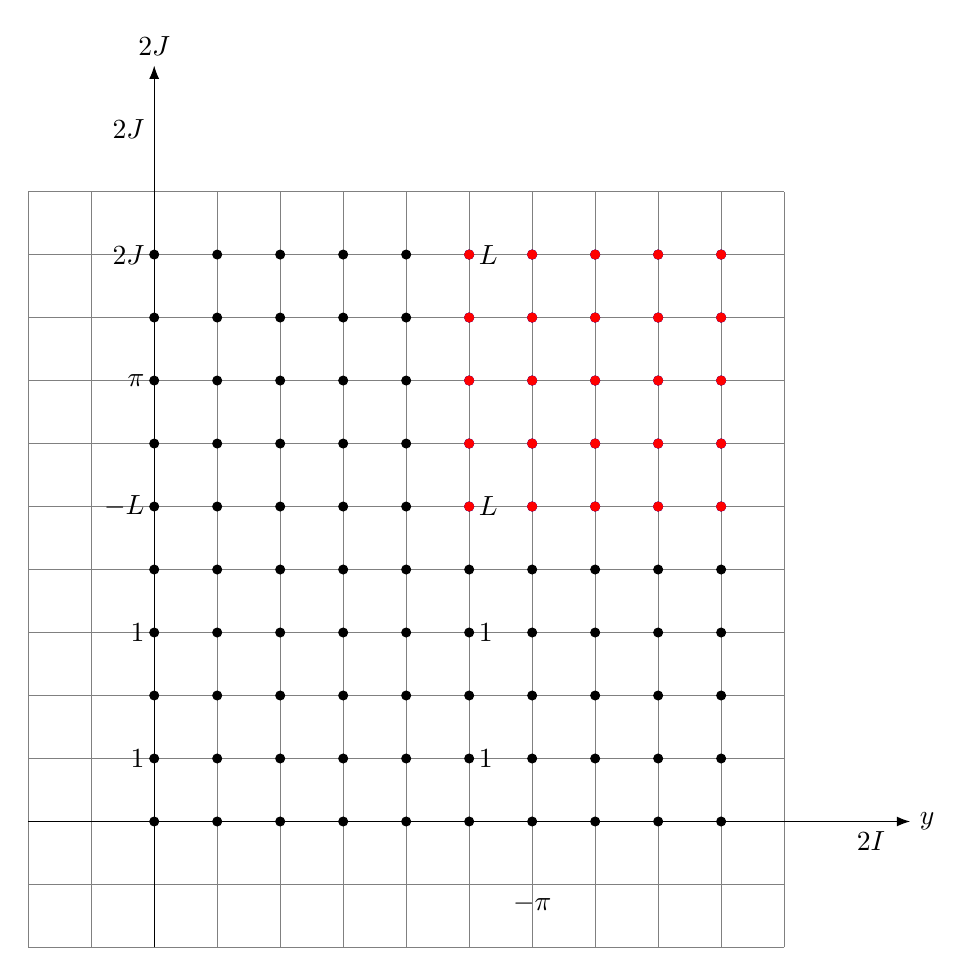
\begin{tikzpicture}[scale=0.8]
    % Draw the grid
    \draw[help lines] (-2,-2) grid (10,10);
    
    % Draw the axes
    \draw[-Latex] (-2,0) -- (12,0) node[right] {$y$};
    \draw[-Latex] (0,-2) -- (0,12) node[above] {$2J$};
    
    % Annotate the axes
    \node at (11,0) [below right] {$2I$};
    \node at (0,11) [left] {$2J$};
    \node at (0,5) [left] {$-L$};
    \node at (0,9) [left] {$2J$};
    \node at (0,7) [left] {$\pi$};
    \node at (0,3) [left] {$1$};
    \node at (0,1) [left] {$1$};
    \node at (6,-1) [below] {$-\pi$};
    
    % Draw the nodes
    \foreach \x in {0,...,9} {
        \foreach \y in {0,...,9} {
            \filldraw[black] (\x,\y) circle (2pt);
        }
    }
    
    \foreach \x in {0,...,4} {
        \foreach \y in {0,...,4} {
            \filldraw[blue] (\x+5,\y+5) circle (2pt);
        }
    }
    
    \foreach \x in {0,...,4} {
        \foreach \y in {0,...,4} {
            \filldraw[red] (\x+5,\y+5) circle (2pt);
        }
    }
    
    % Annotate the boundary conditions
    \node at (5,5) [right] {$L$};
    \node at (5,9) [right] {$L$};
    \node at (5,1) [right] {$1$};
    \node at (5,3) [right] {$1$};
    
\end{tikzpicture}

\end{document}